\documentclass[tikz]{standalone}
\usepackage{pgfplots}
\pgfplotsset{compat=1.15}
\usepackage{mathrsfs}
\usetikzlibrary{arrows,calc}
\usepackage{tkz-euclide}
\pagestyle{empty}

\definecolor{AngleClr}{rgb}{0,0.39215686274509803,0}
\definecolor{ShapeClr}{rgb}{0.6,0.2,0}
\definecolor{SquareClr}{RGB}{250, 248, 217}
\definecolor{GreenDist}{RGB}{7,122,7}

\begin{document}

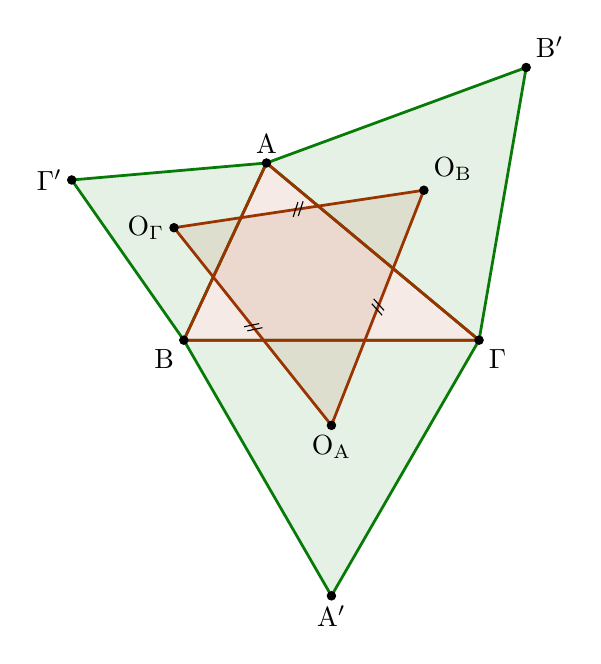
\begin{tikzpicture}[scale=.75]
\tkzSetUpLine[line width=1pt,color=black]
\tkzSetUpPoint[fill=black]

\tkzDefPoints{0/0/B,1.4/3/A,5/0/C}

\tkzDefTriangle[equilateral](C,B) \tkzGetPoint{A'}
\tkzDefTriangle[equilateral](A,C) \tkzGetPoint{B'}
\tkzDefTriangle[equilateral](B,A) \tkzGetPoint{C'}


\tkzDefTriangleCenter[circum](A',B,C) \tkzGetPoint{OA}
\tkzDefTriangleCenter[circum](A,B',C) \tkzGetPoint{OB}
\tkzDefTriangleCenter[circum](A,B,C') \tkzGetPoint{OC}


\tkzFillPolygon[fill=ShapeClr,fill opacity=0.1](A,B,C)
\tkzFillPolygon[fill=GreenDist,fill opacity=0.1](A',B,C)
\tkzFillPolygon[fill=GreenDist,fill opacity=0.1](A,B',C)
\tkzFillPolygon[fill=GreenDist,fill opacity=0.1](A,B,C')
\tkzFillPolygon[fill=ShapeClr,fill opacity=0.1](OA,OB,OC)

\tkzDrawPolygons[color=GreenDist](A',B,C A,B',C A,B,C')
\tkzDrawPolygon[color=ShapeClr](A,B,C)
\tkzDrawPolygon[color=ShapeClr](OA,OB,OC)

\tkzDrawPoints[size=3](A,B,C,A',B',C',OA,OB,OC)

\tkzLabelPoint[above](A){$\rm A$}
\tkzLabelPoint[below left](B){$\rm B$}
\tkzLabelPoint[below right](C){$\rm \Gamma$}

\tkzLabelPoint[left](C'){$\rm \Gamma'$}
\tkzLabelPoint[above right](B'){$\rm B'$}
\tkzLabelPoint[below](A'){$\rm A'$}

\tkzLabelPoint[left](OC){$\rm O_\Gamma$}
\tkzLabelPoint[above right](OB){$\rm O_B$}
\tkzLabelPoint[below](OA){$\rm O_A$}

\tkzMarkSegments[mark=s||,size=2.5](OA,OB OB,OC OC,OA)

\end{tikzpicture}

\end{document}
